\chapter{Case Study} \label{chap:casestudy}

\section*{}

In this chapter we present two case studies that were used as a proof of concept
for the developed system. We characterize the experimental environment, the used
data sets and the obtained results for both cases. We then compare the developed
solutions with the previously available methods.

\section{Gene Expression Analysis Pipeline}

This case study is aimed at the developed gene expression pipeline, composed by
iRAP and the differential expression results combination tool. Gene expression
analysis is a complex task and, because of that, no definitive tool exists that
can produce good results for every possible case. Some tools are better when
analysing certain types of data/organisms, while other tools might have other
strengths and weaknesses. It is difficult to an inexperienced user, as it is to
a computer system, to determine the best tool to use in each case. The objective
of this case study is to ascertain if the developed pipeline enhancement can
help overcome this difficult, by combining the best results from multiple tools.

\subsection{Case Study Setup}

The data used in this case study was obtained from Ensembl Genomes (annotated
reference genome) and ENA Sequence Read Archive (sequencing reads). The
experiment itself is based on RNA-Seq experiment
\emph{E-GEOD-48829},
available at ArrayExpress\footnote{ArrayExpress in an online database where
researchers can submit and search functional genomics experiments. This
particular experience can be found at \url{http://www.ebi.ac.uk/arrayexpress/experiments/E-GEOD-48829/}.}.

\subsubsection*{Analysis Data Set}

As previously mentioned, the used data set was the same as in ArrayExpress
experiment \emph{E-GEOD-48829}. This experiment studies the \emph{Escherichia
coli} bacteria, commonly known as \emph{E. coli}. \emph{E. coli} is a model
organism: a \qt{simple}, non-human organism that is extensively studied, with
the expectation that the discoveries made for that particular organism are
useful to understand different organisms \cite{fields2005cell}. Other examples
of model organisms are \emph{Rattus norvegicus} (norway rat), \emph{Drosophila
melanogaster} (fruit fly) and \emph{Mus musculus} (common mouse).

Being extensively studied was just one of the reasons that lead to this choice
of data set. As a single cellular organism, \emph{E. coli} is a simple organism,
whose genome is fairly short (when compared with vertebrates, for example). This
allows for much faster analysis times of a few hours, as opposed to the longer
run times of larger genomes.

The experiment was composed by a total of six libraries. These libraries where
divided into two groups. These groups were used to define a contrast\footnote{In
the context of differential expression a contrast is composed by two groups of
libraries; these groups are compared between them, in order to uncover
differences in their expression levels.} in the differential expression
analysis.

\subsubsection*{Experimental Environment}

For this data set all tests were performed in the same machine. The machine's
specifications can be consulted in Table \ref{tab:specs_irap}. Performance was
not a big concern in this case study, as it is expected that iRAP may takes
between hours and days to complete an experiment. In these experiments the
biggest constraint is the machine's memory: older machines might not have enough
memory to execute a complex iRAP analysis.

\begin{table}[!htb]
  \centering
  \begin{tabular}{{l} | {l}{l}}
    & \textbf{\emph{Machine}}\\ \hline
    \textbf{\emph{Operative system}}    & Debian GNU/Linux Jessie/Sid\\
    \textbf{\emph{CPU}}                 & Intel Core 2 Quad Q9400 (4 cores)\\
    \textbf{\emph{CPU speed}}           & 2.66 GHz\\
    \textbf{\emph{Memory}}              & 16 GiB DDR2 (800 MHz) \\ \hline
  \end{tabular}

  \caption[Specifications of the test environment used for the case study experiments]{
    Specifications of the test environment used for the case study experiments.
  }
  \label{tab:specs_irap}
\end{table}

\subsubsection*{Methodology}

Firstly, all information related to the experiment was download to the test
machine (annotated reference genome and reads). A configuration file for the
experiment was written, defining settings, libraries, groups, contrasts and any
other information relevant to the experiment.

The experiment was then executed until the quantification step; no differential
expression analysis was performed at this point. This preliminary experiment
used TopHat as a mapping/alignment tool and HTSeq as a quantification tool (see
Section \ref{sec:seqtools}).

Differential expression analysis was then performed using the previously
produced quantification data. This analysis was conducted with both edgeR and
DESeq (see Section \ref{sec:difexptools}). The total number of distinct lines in
each result file was counted (for both tools). The next step was to remove any
entries with high \emph{p-values} from those files, leaving only lines with a
\emph{p-value} less or equal to 0.05. New line counts were produced for each of
the filtered files. Finally, both files were combined in a single using the
produced tool, and a last line count was made.

\subsection{Comparison with Previous Results}

The developed tool's results were compared with both the normal \qt{raw} results
directly produced by the differential expression tools and with those same
results, filtered by \emph{p-value}. Table \ref{tab:test_irap} shows these
results, in terms of distinct lines per results file. Note that every line
corresponds to a unique differentially expressed gene.

\begin{table}[!htb]
  \centering
  \begin{tabular}{{l} | {c}{c}{c}}
    & \textbf{\emph{Raw results}} & \textbf{\emph{Filtered results}} & \textbf{\emph{Combined results}}\\ \hline
    \textbf{\emph{edgeR}} & 4494 & 386 & \multirow{2}{*}{191}\\
    \textbf{\emph{DESeq}} & 4494 & 204 \\ \hline
  \end{tabular}

  \caption[Number of distinct lines resulting from differential expression analysis]{
    Number of distinct lines resulting from differential expression analysis.
    These results are relative to the raw results produced by the differential
    expression tools, those same results filtered by \emph{p-value} and combined
    with the produced tool.
  }
  \label{tab:test_irap}
\end{table}

This experiment demonstrates that the developed tool can in fact filter the
results of differential expression into a smaller data set. This filtered data
set will hopefully reveal itself more useful to researchers, eliminating
unnecessary information and giving higher levels of confidence in the results.
However, we have no way of comparing these results with the previous ones from a
biological standpoint. Such assessment must be performed by expert in this
field, which was not possible at this time.

\section{RNA Binding Protein Analysis Web Platform}

This case study is aimed at the RBP analysis tool (PBS Finder).
\emph{RhoGTPases} comprise a family of molecular switches that control signal
transduction pathways that link cell surface receptors to a variety of
intracellular responses. In this particular case the genes are related to the
well known model organism \emph{Rattus norvegicus}, commonly known as
\emph{norway rat}. This data set was produced by IBMC experts. The same experts
then validated the obtained results experimentally. The same experts then
validated the obtained results experimentally.

This experiment has three distinct goals. The first goal is to assess the
general usefulness of PBS Finder. It is important to determine if the developed
tool can at least reproduce the results obtained with previous methods. It is
also relevant to assess if PBS Finder is able to provide even more relevant
information to researchers, facilitating their work. The second goal is to
compare PBS Finder with the existing techniques of manual analysis. One of the
major constraints of manual analysis is the time it takes to complete; PBS
Finder should be able to reduce the duration of the analysis. Lastly, the third
goal is to assess the impact of differences in hardware performance in the
overall performance of the platform. PBS Finder should be sufficiently optimized
to be able to run in personal computers with decreased hardware performance,
instead of only in servers/computer clusters.

\subsection{Case Study Setup}

The available case study data set was produced by IBMC experts. The same experts
then validated the obtained results experimentally. The same experts then
validated the obtained results experimentally.

\subsubsection*{Analysis Data Set}

The analysis data set is comprised by twenty three gene identifiers, from the
\emph{RhoGTPase} family. The actual genes used for our tests can be found in
Table \ref{tab:genes}. Note that the tool only needs to receive gene
identifiers; gene names are not currently accepted as input data.

\begin{table}[!htb]
  \centering
  \begin{tabular}{{l}{l}{l}}
    \textbf{\emph{Gene name}} & \textbf{\emph{Gene ID}} & \textbf{\emph{Transcript ID}}\\ \hline
    Rhoj        & ENSRNOG00000021919 & ENSRNOT00000031979\\
    Rhog        & ENSRNOG00000020393 & ENSRNOT00000027641\\
    Rac3        & ENSRNOG00000048172 & ENSRNOT00000073886\\
    Rac2        & ENSRNOG00000007350 & ENSRNOT00000009994\\
    Rhod        & ENSRNOG00000019220 & ENSRNOT00000026092\\
    Rhof        & ENSRNOG00000042607 & ENSRNOT00000064390\\
    Rhoh        & ENSRNOG00000002540 & ENSRNOT00000003425\\
    Rnd         & ENSRNOG00000020698 & ENSRNOT00000028089\\
    Rhoc        & ENSRNOG00000012630 & ENSRNOT00000017254\\
    Cdc42       & ENSRNOG00000013536 & ENSRNOT00000029025\\
    Cdc42       & ENSRNOG00000013536 & ENSRNOT00000018118\\
    Rhoq        & ENSRNOG00000015415 & ENSRNOT00000020822\\
    Rac1        & ENSRNOG00000001068 & ENSRNOT00000001417\\
    Rhou        & ENSMUSG00000039960 & ENSMUST00000136615\\
    Rhou        & ENSMUSG00000039960 & ENSMUST00000045487\\
    Rhoa        & ENSRNOG00000050519 & ENSRNOT00000071664\\
    Rnd1        & ENSRNOG00000013621 & ENSRNOT00000018276\\
    Rnd3        & ENSRNOG00000004624 & ENSRNOT00000006111\\
    Rhob        & ENSRNOG00000021403 & ENSRNOT00000008008\\
    Rhobtb1     & ENSRNOG00000000633 & ENSRNOT00000000784\\
    Rhobtb2     & ENSRNOG00000017373 & ENSRNOT00000023876\\
    Rhobtb3     & ENSRNOG00000012414 & ENSRNOT00000016838\\
    Rhov        & ENSRNOG00000013380 & ENSRNOT00000018277\\ \hline
  \end{tabular}

  \caption[\emph{RhoGTPase} family genes used as data set in the case study]{
    \emph{RhoGTPase} family genes used as data set in the case study.
  }
  \label{tab:genes}
\end{table}

\subsubsection*{Experimental Environment}

The testing environment was reproduced in two different machines. This machines
differ in their hardware and operative system, but every other variable in the
environment (internet connection speeds, machine usage, etc.) holds for both
machines. Performance results for the case study experiment for both machines
are given in Section \ref{sec:caseperf}. Henceforth the machines will be
referenced as \emph{Machine1} and \emph{Machine2}, as shown in Table
\ref{tab:specs}.

\begin{table}[!htb]
  \centering
  \begin{tabular}{{l} | {l}{l}}
    & \textbf{\emph{Machine1}} & \textbf{\emph{Machine2}}\\ \hline
    \textbf{\emph{Operative system}}    & OS X 10.9.3                     & Debian GNU/Linux Jessie/Sid\\
    \textbf{\emph{CPU}}                 & Intel Core i7 4850HQ (4 cores)  & Intel Core 2 Quad Q9400 (4 cores)\\
    \textbf{\emph{CPU speed}}           & 2.30 GHz                        & 2.66 GHz\\
    \textbf{\emph{Memory}}              & 16 GiB DDR3 (1600 MHz)          & 16 GiB DDR2 (800 MHz) \\
    \textbf{\emph{Internet connection}} & 100 Mbps                        & 100 Mbps\\ \hline
  \end{tabular}

  \caption[Specifications of the test environments used for the case study experiments]{
    Specifications of the test environments used for the case study experiments.
  }
  \label{tab:specs}
\end{table}

\subsubsection*{Methodology}

In order for the experiments' execution time to depend only on the hardware of
the machines several environment restrictions were enforced. Firstly, it was
ensured that both machines were running their operative systems with the minimum
required applications, without any parallel usage. The network connections were
also checked to assert if they were working at equal speeds. Lastly, both
machines were verified in order to ascertain if all needed software had equal or
equivalent versions.

Ten experiments ran on each machine. These experiments were executed
sequentially rather than concurrently, to ensure more consistent results. Note
that access to the tool was barred to other users during these experiments for
the same reason. It was also ensured that the support structures of the
platform, including databases, were only used for this set of experiments and
reseted after each one.

\subsection{Results}

Table \ref{tab:results} includes the relevant results for this case study. As
expected, some RBPs are able to bind to almost all members of the
\emph{RhoGTPase} family (for example \emph{Muscleblind-Like Splicing Regulator
1} (MBNL1)), where others were more specific (for example \emph{Y Box Binding
Protein 1} (YBX1)). The latter kind is more interesting to analyse, as it might
be used to manipulate a very specific set of genes, while leaving all others
unaltered. In this case we chose the RBP YBX1 as the base of our validation,
both because it only interacts with five genes and because the genes it
interacts with are representative of the data set, in terms of biological
classification.

\begin{table}[!htb]
  \tiny
  \begin{tabular}{{l}{l} | {c}{c}{c}{c}{c}{c}{c}{c}{c}{c}{c}{c}}
    & & \textbf{\emph{SNRPA}} & \textbf{\emph{ELAVL2}} & \textbf{\emph{HNRNPA1}} & \textbf{\emph{NONO}} & \textbf{\emph{PABPC1}} & \textbf{\emph{ZRANB2}} & \textbf{\emph{RBMY1A1}} & \textbf{\emph{FUS}} & \textbf{\emph{PUM2}} & \textbf{\emph{SFRS9}} & \textbf{\emph{MBNL1}} & \textbf{\emph{EIF4B}}\\ \hline
    \parbox[t]{2mm}{\multirow{9}{*}{\rotatebox[origin=c]{90}{\emph{Cluster 1}}}}
    & \textbf{\emph{Rhoj}} &  &  &  & $\times$ & $\times$ &  & $\times$ & $\times$ & $\times$ & $\times$ & $\times$ & $\times$\\
    & \textbf{\emph{Rhog}} &  &  &  & $\times$ & $\times$ &  & $\times$ &  &  & $\times$ & $\times$ & $\times$\\
    & \textbf{\emph{Rac3}} &  &  & $\times$ & $\times$ & $\times$ &  & $\times$ & $\times$ & $\times$ & $\times$ & $\times$ & $\times$\\
    & \textbf{\emph{Rac2}} &  &  &  & $\times$ & $\times$ &  & $\times$ & $\times$ &  &  & $\times$ & $\times$\\
    & \textbf{\emph{Rhod}} &  &  & $\times$ &  & $\times$ &  &  & $\times$ & $\times$ & $\times$ & $\times$ & $\times$\\
    & \textbf{\emph{Rhof}} &  &  &  & $\times$ & $\times$ &  &  & $\times$ & $\times$ & $\times$ & $\times$ & $\times$\\
    & \textbf{\emph{Rhoh}} &  &  &  &  &  &  & $\times$ &  & $\times$ & $\times$ & $\times$ & $\times$\\
    & \textbf{\emph{Rnd2}} &  &  &  & $\times$ &  &  &  & $\times$ & $\times$ & $\times$ & $\times$ & $\times$\\
    & \textbf{\emph{Rhoc}} & $\times$ &  & $\times$ & $\times$ &  &  &  & $\times$ & $\times$ & $\times$ & $\times$ & $\times$\\ \\ \hline \\
    \parbox[t]{2mm}{\multirow{14}{*}{\rotatebox[origin=c]{90}{\emph{Cluster 2}}}}
    & \textbf{\emph{Cdc42}} & $\times$ & $\times$ & $\times$ & $\times$ & $\times$ & $\times$ & $\times$ & $\times$ & $\times$ & $\times$ & $\times$ & $\times$\\
    & \textbf{\emph{Cdc42}} &  & $\times$ &  & $\times$ &  &  & $\times$ & $\times$ & $\times$ & $\times$ & $\times$ & $\times$\\
    & \textbf{\emph{Rhoq}} & $\times$ &  &  & $\times$ & $\times$ &  & $\times$ & $\times$ & $\times$ & $\times$ & $\times$ & $\times$\\
    & \textbf{\emph{Rac1}} & $\times$ &  &  &  & $\times$ &  &  & $\times$ & $\times$ & $\times$ & $\times$ & $\times$\\
    & \textbf{\emph{Rhou}} &  &  &  &  &  &  &  &  &  &  &  & \\
    & \textbf{\emph{Rhou}} & $\times$ & $\times$ & $\times$ & $\times$ & $\times$ &  & $\times$ & $\times$ & $\times$ & $\times$ & $\times$ & $\times$\\
    & \textbf{\emph{Rhoa}} &  & $\times$ &  &  & $\times$ &  &  & $\times$ & $\times$ & $\times$ & $\times$ & $\times$\\
    & \textbf{\emph{Rnd1}} &  &  &  & $\times$ & $\times$ &  &  & $\times$ &  & $\times$ & $\times$ & $\times$\\
    & \textbf{\emph{Rnd3}} &  & $\times$ &  & $\times$ & $\times$ &  & $\times$ & $\times$ & $\times$ & $\times$ & $\times$ & $\times$\\
    & \textbf{\emph{Rhob}} & $\times$ & $\times$ &  & $\times$ & $\times$ &  & $\times$ & $\times$ & $\times$ & $\times$ & $\times$ & $\times$\\
    & \textbf{\emph{Rhobtb1}} & $\times$ & $\times$ & $\times$ & $\times$ & $\times$ & $\times$ & $\times$ & $\times$ & $\times$ & $\times$ & $\times$ & $\times$\\
    & \textbf{\emph{Rhobtb2}} &  &  &  & $\times$ &  &  &  & $\times$ & $\times$ & $\times$ & $\times$ & $\times$\\
    & \textbf{\emph{Rhobtb3}} & $\times$ & $\times$ & $\times$ & $\times$ & $\times$ & $\times$ & $\times$ & $\times$ & $\times$ & $\times$ & $\times$ & $\times$\\
    & \textbf{\emph{Rhov}} &  &  &  & $\times$ & $\times$ &  & $\times$ & $\times$ & $\times$ & $\times$ & $\times$ & $\times$\\ \hline
  \end{tabular}

  \vspace{0.4cm}

  \begin{tabular}{{l}{l} | {c}{c}{c}{c}{c}{c}{c}{c}{c}{c}{c}{c}}
    & & \textbf{\emph{EIF4B}} & \textbf{\emph{KHSRP}} & \textbf{\emph{YTHDC1}} & \textbf{\emph{VTS1}} & \textbf{\emph{RBMX}} & \textbf{\emph{KHDRBS3}} & \textbf{\emph{SFRS1}} & \textbf{\emph{ELAVL1}} & \textbf{\emph{SFRS13A}} & \textbf{\emph{SFRS7}} & \textbf{\emph{A2BP1}} & \textbf{\emph{QKI}}\\ \hline
    \parbox[t]{2mm}{\multirow{9}{*}{\rotatebox[origin=c]{90}{\emph{Cluster 1}}}}
    & \textbf{\emph{Rhoj}} & $\times$ & $\times$ & $\times$ & $\times$ & $\times$ & $\times$ & $\times$ & $\times$ & $\times$ &  & $\times$ & $\times$\\
    & \textbf{\emph{Rhog}} & $\times$ & $\times$ & $\times$ &  & $\times$ & $\times$ & $\times$ & $\times$ & $\times$ &  &  & $\times$\\
    & \textbf{\emph{Rac3}} & $\times$ & $\times$ & $\times$ & $\times$ & $\times$ & $\times$ & $\times$ & $\times$ & $\times$ &  & $\times$ & $\times$\\
    & \textbf{\emph{Rac2}} & $\times$ & $\times$ & $\times$ &  & $\times$ & $\times$ & $\times$ & $\times$ & $\times$ &  &  & \\
    & \textbf{\emph{Rhod}} & $\times$ & $\times$ & $\times$ & $\times$ & $\times$ & $\times$ & $\times$ & $\times$ & $\times$ &  & $\times$ & $\times$\\
    & \textbf{\emph{Rhof}} & $\times$ & $\times$ & $\times$ & $\times$ & $\times$ & $\times$ & $\times$ & $\times$ & $\times$ &  &  & $\times$\\
    & \textbf{\emph{Rhoh}} & $\times$ & $\times$ &  &  & $\times$ & $\times$ & $\times$ & $\times$ & $\times$ &  &  & \\
    & \textbf{\emph{Rnd2}} & $\times$ & $\times$ & $\times$ & $\times$ & $\times$ & $\times$ & $\times$ & $\times$ & $\times$ &  & $\times$ & \\
    & \textbf{\emph{Rhoc}} & $\times$ & $\times$ & $\times$ & $\times$ & $\times$ & $\times$ & $\times$ & $\times$ & $\times$ &  & $\times$ & \\ \\ \hline \\
    \parbox[t]{2mm}{\multirow{14}{*}{\rotatebox[origin=c]{90}{\emph{Cluster 2}}}}
    & \textbf{\emph{Cdc42}} & $\times$ & $\times$ & $\times$ & $\times$ & $\times$ & $\times$ & $\times$ & $\times$ & $\times$ & $\times$ & $\times$ & $\times$\\
    & \textbf{\emph{Cdc42}} & $\times$ & $\times$ & $\times$ &  & $\times$ & $\times$ & $\times$ & $\times$ & $\times$ &  & $\times$ & $\times$\\
    & \textbf{\emph{Rhoq}} & $\times$ & $\times$ & $\times$ & $\times$ & $\times$ & $\times$ & $\times$ & $\times$ & $\times$ &  & $\times$ & $\times$\\
    & \textbf{\emph{Rac1}} & $\times$ & $\times$ & $\times$ & $\times$ & $\times$ & $\times$ & $\times$ & $\times$ & $\times$ &  &  & $\times$\\
    & \textbf{\emph{Rhou}} &  &  &  &  &  &  &  &  &  &  &  & \\
    & \textbf{\emph{Rhou}} & $\times$ & $\times$ & $\times$ & $\times$ & $\times$ & $\times$ & $\times$ & $\times$ & $\times$ &  & $\times$ & \\
    & \textbf{\emph{Rhoa}} & $\times$ & $\times$ & $\times$ & $\times$ & $\times$ & $\times$ & $\times$ & $\times$ & $\times$ &  &  & $\times$\\
    & \textbf{\emph{Rnd1}} & $\times$ & $\times$ &  & $\times$ & $\times$ & $\times$ & $\times$ & $\times$ & $\times$ &  & $\times$ & \\
    & \textbf{\emph{Rnd3}} & $\times$ & $\times$ & $\times$ & $\times$ & $\times$ & $\times$ & $\times$ & $\times$ & $\times$ &  & $\times$ & \\
    & \textbf{\emph{Rhob}} & $\times$ & $\times$ & $\times$ & $\times$ & $\times$ & $\times$ & $\times$ & $\times$ & $\times$ & $\times$ & $\times$ & \\
    & \textbf{\emph{Rhobtb1}} & $\times$ & $\times$ & $\times$ & $\times$ & $\times$ & $\times$ & $\times$ & $\times$ & $\times$ &  & $\times$ & \\
    & \textbf{\emph{Rhobtb2}} & $\times$ & $\times$ &  & $\times$ & $\times$ &  & $\times$ & $\times$ & $\times$ &  &  & \\
    & \textbf{\emph{Rhobtb3}} & $\times$ & $\times$ & $\times$ & $\times$ & $\times$ & $\times$ & $\times$ & $\times$ & $\times$ &  & $\times$ & $\times$\\
    & \textbf{\emph{Rhov}} & $\times$ & $\times$ & $\times$ & $\times$ & $\times$ & $\times$ & $\times$ & $\times$ & $\times$ &  &  & \\ \hline
  \end{tabular}

  \vspace{0.4cm}

  \begin{tabular}{{l}{l} | {c}{c}{c}{c}{c}{c}{c}{c}{c}{c}{c}{c}}
    & & \textbf{\emph{QKI}} & \textbf{\emph{SUS}} & \textbf{\emph{YBX2-A}} & \textbf{\emph{PSI}} & \textbf{\emph{SAP-49}} & \textbf{\emph{ACO1}} & \textbf{\emph{YBX1}} & \textbf{\emph{SFRS2}} & \textbf{\emph{ZFP36}} & \textbf{\emph{RBM4}} & \textbf{\emph{PTBP1}}\\ \hline
    \parbox[t]{2mm}{\multirow{9}{*}{\rotatebox[origin=c]{90}{\emph{Cluster 1}}}}
    & \textbf{\emph{Rhoj}} & $\times$ &  & $\times$ &  & $\times$ &  & $\times$ & $\times$ &  &  & \\
    & \textbf{\emph{Rhog}} & $\times$ &  &  &  &  & $\times$ &  &  &  &  & \\
    & \textbf{\emph{Rac3}} & $\times$ &  &  &  &  &  &  &  &  &  & \\
    & \textbf{\emph{Rac2}} &  &  & $\times$ &  &  &  &  &  &  &  & \\
    & \textbf{\emph{Rhod}} & $\times$ &  &  &  &  &  &  &  &  &  & \\
    & \textbf{\emph{Rhof}} & $\times$ &  &  &  &  & $\times$ &  & $\times$ &  & $\times$ & \\
    & \textbf{\emph{Rhoh}} &  &  &  &  &  &  &  &  &  &  & \\
    & \textbf{\emph{Rnd2}} &  &  &  &  &  & $\times$ &  & $\times$ &  &  & \\
    & \textbf{\emph{Rhoc}} &  &  &  &  &  &  &  &  &  &  & \\ \\ \hline \\
    \parbox[t]{2mm}{\multirow{14}{*}{\rotatebox[origin=c]{90}{\emph{Cluster 2}}}}
    & \textbf{\emph{Cdc42}} & $\times$ &  &  &  &  &  &  &  &  &  & \\
    & \textbf{\emph{Cdc42}} & $\times$ & $\times$ & $\times$ & $\times$ & $\times$ & $\times$ & $\times$ &  &  &  & \\
    & \textbf{\emph{Rhoq}} & $\times$ &  & $\times$ &  & $\times$ & $\times$ &  &  & $\times$ & $\times$ & \\
    & \textbf{\emph{Rac1}} & $\times$ &  & $\times$ &  & $\times$ & $\times$ &  &  &  & $\times$ & \\
    & \textbf{\emph{Rhou}} &  &  &  &  &  &  &  &  &  &  & \\
    & \textbf{\emph{Rhou}} &  &  & $\times$ &  & $\times$ & $\times$ &  &  & $\times$ &  & \\
    & \textbf{\emph{Rhoa}} & $\times$ &  &  &  & $\times$ & $\times$ & $\times$ &  &  & $\times$ & \\
    & \textbf{\emph{Rnd1}} &  &  &  &  &  & $\times$ &  &  & $\times$ &  & \\
    & \textbf{\emph{Rnd3}} &  &  &  & $\times$ & $\times$ & $\times$ & $\times$ &  &  &  & $\times$\\
    & \textbf{\emph{Rhob}} &  &  &  &  & $\times$ & $\times$ &  &  &  & $\times$ & \\
    & \textbf{\emph{Rhobtb1}} &  &  &  &  &  & $\times$ & $\times$ &  &  & $\times$ & \\
    & \textbf{\emph{Rhobtb2}} &  &  & $\times$ &  &  & $\times$ &  &  &  &  & \\
    & \textbf{\emph{Rhobtb3}} & $\times$ &  & $\times$ &  & $\times$ & $\times$ &  & $\times$ & $\times$ &  & \\
    & \textbf{\emph{Rhov}} &  &  &  &  & $\times$ & $\times$ &  &  &  &  & \\ \hline
  \end{tabular}

  \caption[Case study results generated by PBS Finder]{
    Case study results generated by PBS Finder (table divided intro three
    sections for legibility). Each row represents a single gene from the data
    set and each row represents an RBP with which the genes potentially bind.
    Note that for this particular analysis the tool divided the genes into two
    clusters, joining together genes that bind with similar proteins.
  }
  \label{tab:results}
\end{table}

Table \ref{tab:results} shows that the tool found two clusters of genes within
the data set. In this case the best results were obtained using average linkage
hierarchical clustering, coupled with a binary representation of the distance
matrix. This particular solution was chosen for having a higher average
silhouette than other produced solutions. Table \ref{tab:differ} contains a list
of all the proteins that were considered as defining for their clusters. Note
that \emph{Cluster 1} contained almost exclusively proteins that were frequent
across the data set; on the other hand, \emph{Cluster 2} contained seven RBPs
that were identified as features of that cluster.

\begin{table}[!htb]
  \centering
  \begin{tabular}{{c} | {l}}
    \textbf{\emph{Cluster 1}} & \textbf{\emph{Cluster 2}}\\ \hline
    \multirow{7}{*}{-}
    & ZFP36 \\
    & ELAVL2 \\
    & ZRANB2 \\
    & PSI \\
    & PTBP1 \\
    & SFRS7 \\
    & SUS \\ \hline
  \end{tabular}

  \caption[RBPs found to characterize each cluster]{
    RBPs found to characterize each cluster. Note that \emph{Cluster 1} does not
    contain any RBP that can be considered as a defining feature of that
    cluster. This is due to the fact that proteins in \emph{Cluster 1} are
    generally abundant through the data set.
  }
  \label{tab:differ}
\end{table}

\subsection{Correctness and Completeness of the Results}\label{sec:caseval}

Result checking was conducted in two different fronts: \emph{collected data
completeness and correction}; and \emph{biological results evaluation}.

Completeness and correction analysis were conducted both manually and
automatically during the development of the tool. In some cases it was possible
to automate these validations using \emph{unit testing}\footnote{Unit testing is
a software testing method that focus on testing individual units of a developed
software; these tests are used to assess which of those units are fit, and which
do not work correctly.} and \emph{mocks}\footnote{A mock, or mock object, is a
simulated object that mimics the behavior of a complex component of a software
system. Mock objects are particularly useful when the behavior of its real
counterpart is hard/costly to predict and control}. However, creating this test
infrastructure is a lengthy process. As such, some results, as is the case with
this case study, were manually validated. This validation involves manually
visiting every website used to collect information and cross reference that
information with the one collected by the tool.

The validation of biological results is more complex. It involves experimentally
obtaining the same information that the tool produces, from biological samples.
This validation was conducted at IBMC. However, it is a lengthy process, as
obtaining this information may take several weeks. It has two main objectives:
validating the number and type of RBPs that bind to each gene; and validate the
adequacy of the gene clustering results.

Both checking processes were conducted successfully, thus improving the
confidence that the developed platform produces adequate results.

\subsection{Comparison with Previous Method}\label{sec:caseperf}

As with any newly developed automation tool, it is essential to assess if the
developed tool is in fact an improvement over previously available methods. The
results produced by the tool were already determined correct in Section
\ref{sec:caseval}. As such, the tool should now be evaluated from the user
experience standpoint, namely, in terms of \emph{task simplification} and
\emph{efficiency}.

\subsubsection*{Task Simplification}

Figure \ref{fig:oldvsnew} depicts how PBS Finder simplified the analysis process,
from the user point of view. When conducting a manual analysis, the user must
individually analyse every gene in the data set.

\begin{figure}[!htb]
  \begin{center}
    \leavevmode
    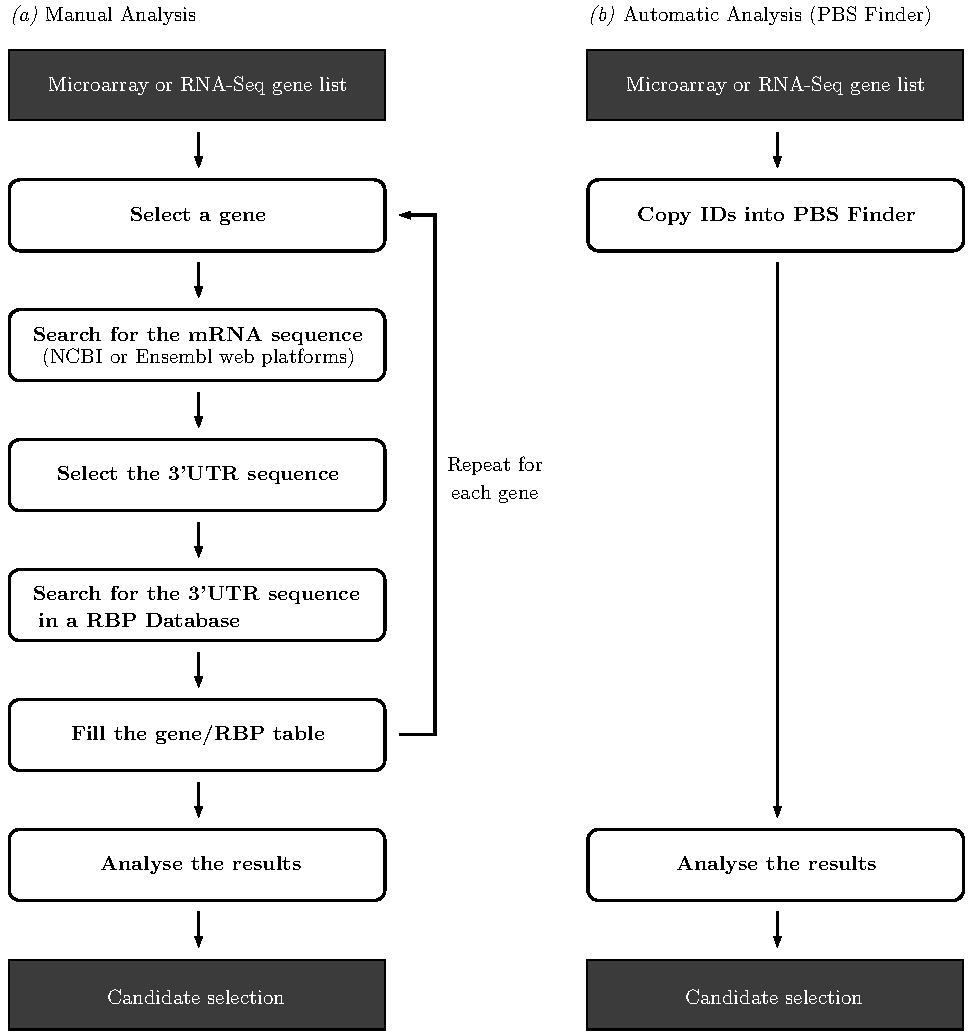
\includegraphics[width=\textwidth]{oldvsnew}
    \caption[Comparison between manual RBP analysis and automatic RBP analysis]{
      Comparison between manual RBP analysis and automatic RBP analysis
      (conducted with PBS Finder).
    }
    \label{fig:oldvsnew}
  \end{center}
\end{figure}

The first step is to select a gene for analysis. The gene identifier is then
searched in either Ensembl or NCBI web platforms, depending on the type of the
identifier. If the gene is found in those platforms, the next step involves
finding the 3'UTR sequence in the results page and copying it. That sequence is
then passed to an online RBP analysis platform, that should retrieve a list of
RBPs that may bind to that particular sequence. Lastly, the RBP information must
be manually combined in the results table. When this information is collected
for every gene it is finally possible to conduct a useful analysis.

On the other hand, with PBS Finder the user needs only to provide the complete
list of all gene identifiers in the data set. The tool will them automatically
process those identifiers, find all relevant information and present it to the
user, ready for further analysis. Note that these results contain additional
information that is not available in the manual analysis: gene, transcript and
protein information (names, additional sequences, pathways, etc.); links to
external platforms; useful histograms; and gene and protein clustering results.

\subsubsection*{Efficiency}

It is essential for the developed platform to be able to conduct the analysis in
a timely fashion, making tool performance a major concern. As such, we compared
the average time that an expert would take to analyse the data set to the
average time that the tool takes to analyse the same data set.

The consulted molecular biology expert estimated that, on average, it would take
thirty minutes to analyse a single gene. This means that an expert would need an
average of eleven and a half hours ($30\ minutes \times 23\ genes$) to process the
entire case study data set.

On the other hand, the automated tool takes a shorter amount of time to conduct
the analysis of the same data set. In order to assess the actual amount of time
the tool took to analyse the entire data set we ran twenty sequential
experiences, ten for each of the experimental environments. Table \ref{tab:perf}
depicts the duration of each one of those experiments, as well as their average
duration. As expected, an automated tool widely outperforms a human expert in
information collection and analysis.

\begin{table}[!htb]
  \centering
  \begin{tabular}{{l} | {l}{l}}
    & \textbf{\emph{Machine1}} & \textbf{\emph{Machine2}}\\ \hline
    \textbf{\emph{Experience 1}}    & $1m\ 47s$ & $6m\ 34s$\\
    \textbf{\emph{Experience 2}}    & $1m\ 58s$ & $6m\ 25s$\\
    \textbf{\emph{Experience 3}}    & $1m\ 46s$ & $6m\ 30s$\\
    \textbf{\emph{Experience 4}}    & $1m\ 45s$ & $6m\ 15s$\\
    \textbf{\emph{Experience 5}}    & $2m\ 23s$ & $6m\ 42s$\\
    \textbf{\emph{Experience 6}}    & $1m\ 35s$ & $6m\ 30s$\\
    \textbf{\emph{Experience 7}}    & $1m\ 40s$ & $6m\ 31s$\\
    \textbf{\emph{Experience 8}}    & $1m\ 39s$ & $6m\ 11s$\\
    \textbf{\emph{Experience 9}}    & $1m\ 42s$ & $6m\ 42s$\\
    \textbf{\emph{Experience 10}}   & $1m\ 42s$ & $6m\ 52s$\\ \hline
    \textbf{\emph{Average time}}    & $1m\ 42s$ & $6m\ 31s$\\ \hline
  \end{tabular}

  \caption[Execution times of the case study data set in two different environments]{
    Execution times of the case study data set in two different environments
    (sequential experiments). Note that while \emph{Machine2} has a significant
    loss in performance (due to its outdated hardware) it still achieves
    satisfactory execution times. This test also shows that it is possible to
    efficiently run PBS Finder in a home computer.
  }
  \label{tab:perf}
\end{table}

Table \ref{tab:stress} contains the stress test results of both machines,
compared to the estimated work time needed by an expert. In this case stress
tests were executed with one hundred, five hundred and nine hundred gene
identifiers. Even the slowest test can be completed by the machine with less
performance (\emph{Machine2}) in under three hours. That same effort would take
an expert approximately four hundred and fifty hours, which amounts to two and a
half weeks on a twenty four hour working day, and to just under two months in
normal working conditions (eight hours per day).

\begin{table}[!htb]
  \centering
  \begin{tabular}{{l} | {l}{l}{l}}
    \textbf{\emph{Number of IDs}} & \textbf{\emph{Machine1}} & \textbf{\emph{Machine2}} & \textbf{\emph{Manual method}} \\ \hline
    100  & $9m\ 56s$          & $11m\ 1s$      & $\approx 50h$\\
    500   & $41m\ 47s$         & $55m\ 51s$     & $\approx 250h$\\
    900   & $1h\ 33m\ 32s$     & $2h\ 7m\ 4s$   & $\approx 450h$\\ \hline
  \end{tabular}

  \caption[Results comparison between manual analysis and both test machines]{
    Results comparison between manual analysis and both test machines.
  }
  \label{tab:stress}
\end{table}

\section{Chapter Conclusions}

The first case study has shown that that the developed tool for result
combination can in fact produce more refined data sets. These filtered and
combined data sets eliminate unnecessary data, and give biologists an higher
level of confidence in the differential expression results.

Through the second case study we have shown that PBS Finder produces relevant
and correct results for large-scale analysis of RBPs using data from \ngs{}
techniques. We have also shown that our tool significantly facilitates the work
of the biologist, by making analysis of this data easier and quicker. As such,
we consider PBS Finder a tool of great value for studying RNA biology.

